% !TEX TS-program = lualatexmk
% glossa-template.tex
% Copyright 2016 Guido Vanden Wyngaerd
%
% This work may be distributed and/or modified under the
% conditions of the LaTeX Project Public License.
% The latest version of this license is in
%   http://www.latex-project.org/lppl.txt
% and version 1.3 or later is part of all distributions of LaTeX
% version 2005/12/01 or later.
%
% This work has the LPPL maintenance status `maintained'.
% 
% The Current Maintainer of this work is 
% Guido Vanden Wyngaerd (guido.vandenwyngaerd@kuleuven.be).
%
% This work consists of the files 
% glossa.cls
% glossa.bst
% gl-authoryear-comp.cbx
% biblatex-gl.bbx
% glossa-template.tex
% glossa.png
%
% The files of the work are derived from the Semantics & Pragmatics style files
% by Kai von Fintel, Christopher Potts, and Chung-chieh Shan
% All changes are documented on the github repository 
% https://github.com/guidovw/Glossalatex.

\PassOptionsToPackage{table}{xcolor}
\documentclass[times,linguex,xcolor]{glossa}
\usepackage{rotating}
\usepackage{tablefootnote}
\usepackage{colortbl}
\usepackage{color}
\usepackage{multicol}
\usepackage{booktabs}

\usepackage{adjustbox}
\usepackage{array}

\newcolumntype{R}[2]{%
    >{\adjustbox{angle=#1,lap=\width-(#2)}\bgroup}%
    l%
    <{\egroup}%
}

\newcommand*\rots{\multicolumn{1}{R{90}{.7em}}}% no optional argument here, please!
%\usepackage{xcolor}

% possible options:
% [times] for Times font (default if no option is chosen)
% [cm] for Computer Modern font
% [lucida] for Lucida font (not freely available)
% [brill] open type font, freely downloadable for non-commercial use from http://www.brill.com/about/brill-fonts; requires xetex
% [charis] for CharisSIL font, freely downloadable from http://software.sil.org/charis/
% for the Brill an CharisSIL fonts, you have to use the XeLatex typesetting engine (not pdfLatex)
% for headings, tables, captions, etc., Fira Sans is used: https://www.fontsquirrel.com/fonts/fira-sans
% [biblatex] for using biblatex (the default is natbib, do not load the natbib package in this file, it is loaded automatically via the document class glossa.cls)
% [linguex] loads the linguex example package
% !! a note on the use of linguex: in glossed examples, the third line of the example (the translation) needs to be prefixed with \glt. This is to allow a first line with the name of the language and the source of the example. See example (2) in the text for an illustration.
% !! a note on the use of bibtex: for PhD dissertations to typeset correctly in the references list, the Address field needs to contain the city (for US cities in the format "Santa Cruz, CA")

%\addbibresource{sample.bib}
% the above line is for use with biblatex
% replace this by the name of your bib-file (extension .bib is required)
% comment out if you use natbib/bibtex

\let\B\relax %to resolve a conflict in the definition of these commands between xyling and xunicode (the latter called by fontspec, called by charis)
\let\T\relax
\usepackage{xyling} %for trees; the use of xyling with the CharisSIL font produces poor results in the branches. This problem does not arise with the packages qtree or forest.
%\usepackage[linguistics]{forest} %for nice trees!


% \pdf* commands provide metadata for the PDF output. ASCII characters only!
\pdfauthor{}
\pdftitle{What is at-issueness?}
\pdfkeywords{}

\title[What is at-issueness?]{What is at-issueness? An experimental comparison of diagnostics\\ 
  % \bigskip \large Word count: 4720
  }
% Optional short title inside square brackets, for the running headers.

\author[]% short form of the author names for the running header. If no short author is given, no authors print in the headers.
{%as many authors as you like, each separated by \AND.
  % \spauthor{Waltraud Paul\\
  % \institute{CRLAO, CNRS-EHESS-INALCO}\\
  % \small{%105, Bd. Raspail, 75005 Paris\\
  % waltraud.paul@ehess.fr}
  % }
  % \AND
  % \spauthor{Guido Vanden Wyngaerd \\
  % \institute{KU Leuven}\\
  % \small{%Warmoesberg 26, 1000 Brussel\\
  % guido.vandenwyngaerd@kuleuven.be}
  % }%
}


%=====================================================================
%=========================== text ===========================

	% punctuation
		\usepackage{csquotes} % for quotation marks

%====================================================================
%=========================== links, references =======================
	% more linguex options for referencing select examples without parentheses
	  \newif\ifparens\parensfalse
	  \makeatletter
	  \renewcommand{\theExNo}{\protect\theExLBr\arabic{ExNo}\protect\theExRBr}
	  \renewcommand{\theSubExNo}{%
	    \hbox{\if@noftnote\protect\theExLBr\Exarabic{ExNo}\firstrefdash
	        \Exalph{SubExNo}\protect\theExRBr
	      \else
	        \protect\theFnExLBr\Exroman{FnExNo}\firstrefdash%
	        \Exalph{SubExNo}\protect\theFnExRBr
	      \fi}}

	  \renewcommand{\theSubSubExNo}{%
	    \hbox{\if@noftnote\protect\theExLBr%
	            \Exarabic{ExNo}\firstrefdash\Exalph{SubExNo}\secondrefdash
	               \Exroman{SubSubExNo}\protect\theExRBr%
	      \else\protect\theFnExLBr\Exroman{FnExNo}\firstrefdash
	                \Exalph{SubExNo}\secondrefdash\Exarabic{SubSubExNo}\protect\theFnExRBr\fi}}%
	  \makeatother
	  \renewcommand\theExLBr{\ifparens\else(\fi}
	  \renewcommand\theExRBr{\ifparens\else)\fi}
	  \newcommand\pref[1]{{\parenstrue\ref{#1}}}

	% in text citation macros
	\newcommand{\citepos}[1]{\citeauthor{#1}'s \citeyear{#1}}
	\newcommand{\citeposs}[1]{\citeauthor{#1}'s}
	\newcommand{\citetpos}[1]{\citeauthor{#1}'s \citeyear{#1}}

	%
	\usepackage{cleveref}


%=====================================================================
%=========================== figures, tables =========================
	% \usepackage{subcaption}
	\usepackage{multirow}

% positive coefficients/difference
\definecolor{purple1}{RGB}{178,24,43}
\definecolor{purple2}{RGB}{239,138,98} 
\definecolor{purple3}{RGB}{253,219,199} 
%\definecolor{yellow4}{RGB}{255,255,204}
%\definecolor{green1}{RGB}{0, 158, 115} % >.95
%\definecolor{green2}{RGB}{55, 185, 141} % .85-.95
%\definecolor{green3}{RGB}{88, 214, 167} % .75-.85
%\definecolor{green4}{RGB}{119, 242, 194} % <.75

% negative coefficients/difference
\definecolor{yellow1}{RGB}{33,102,172}
\definecolor{yellow2}{RGB}{103,169,207}
\definecolor{yellow3}{RGB}{209,229,240}
%\definecolor{purple4}{RGB}{236,206,223}

\begin{document}


\maketitle


\begin{abstract}
  At-issueness is a key concept in theoretical semantics/pragmatics, but there is no consensus about how it is defined or diagnosed (e.g., \citealt{tonhauser_diagnosing_2012,tonhauser_how_2018,koev_notions_2018}). We present experimental data investigating whether four widely used diagnostics for at-issueness yield consistent results. Our findings reveal significant differences across diagnostics, indicating they are not interchangeable. Since the diagnostics target distinct theoretical conceptions of at-issueness, these differences offer insight into their comparability.

\end{abstract}

% \begin{keywords}
%   at-issueness, experimental pragmatics, discourse interpretation
% \end{keywords}

\section{Introduction \label{sec:1_introduction}}
  At-issueness is a key concept in theoretical semantics and pragmatics, distinguishing between at-issue propositions conveyed by an utterance, those contributing to its main point, and those that do not (e.g., \citealt{karttunen_conventional_1979,horton_presuppositions_1988,abbott_presuppositions_2000,faller_semantics_2003,potts_logic_2005,tonhauser_diagnosing_2012}). Despite its importance, the concept lacks a unified definition. Instead, various theoretical notions (\citealt{koev_notions_2018,tonhauser_how_2018}) and empirical diagnostics (e.g., \citealt{tonhauser_diagnosing_2012}) have been proposed. This paper addresses the question whether four widely used diagnostics for at-issueness yield consistent results when testing the same stimuli. Our findings reveal significant differences across diagnostics, indicating they are not interchangeable. Since the diagnostics target distinct theoretical conceptions of at-issueness, these differences offer insight into their comparability.

  % Do the results support the notion that different theoretical conceptions of at-issueness are distinct?

  The four diagnostics we tested are illustrated in (\pref{qud}--\pref{yesbut}) for sentence-medial non-restrictive relative clauses (NRRCs), which are usually taken to contribute non-at-issue content.  As appositive content is generally taken to be not-at-issue, participants are expected to: Give low naturalness ratings under the QUD diagnostic \ref{qud} and the direct dissent diagnostic \ref{dd}, not interpret the speaker to be asking about the content under the `asking-whether' diagnostic in \ref{aw}, will choose one of the \emph{yes}-responses under the `yes, but' diagnostic in \ref{yesbut}.

  \ex. \label{qud}%
    QUD diagnostic (e.g., \citealt{tonhauser_diagnosing_2012,chen_presuppositions_2024})
    \a.[A:] \emph{What did Greg buy?}
    \b.[B:] \emph{Greg, who bought a new car, is envied by his neighbor.}
    \z.
    Question to participants: How well does B's response fit A's question?
  \z.

  \ex. \label{aw}%
    `asking whether' diagnostic (e.g., \citealt{tonhauser_how_2018,solstad_cataphoric_2024})\smallskip\\
      \emph{Is Greg, who bought a new car, envied by his neighbor?}\smallskip
  \\ Question to participants: Is the speaker asking whether Greg bought a new car?
  \z.

  \ex. \label{dd} Direct dissent diagnostic (e.g., \citealt{tonhauser_diagnosing_2012,syrett_experimental_2015})
    \a.[A:] \emph{Greg, who bought a new car, is envied by his neighbor.}
    \b.[B:]\emph{No, that's not true, he didn't buy a new car.}
    \z.
  Question to participants: How natural is B's rejection of A's utterance?
  \z.

  \ex. \label{yesbut}%
    `yes, but' diagnostic (e.g., \citealt{xue_correlation_2011,destruel_cross-linguistic_2015})
    \a.[A:] \emph{Greg, who bought a new car, is envied by his neighbor.}
    \b.[B:] \emph{Yes, but he didn't buy a new car.} /
    \b.[] \emph{Yes, and he didn't buy a new car.} /
    \b.[] \emph{No, he didn't buy a new car.}
    \z.
    Task for participants: Choose the response that sounds best.
  \z.

  The diagnostics reflect different theoretical conceptions of at-issueness (\citealt{koev_notions_2018}), and they have led to different empirical results, discussed below.


  \subsection{QUD-based diagnostics}
    The diagnostics in \ref{qud} and \ref{aw} are based on the assumption that discourse is organized around addressing a question under discussion (QUD) (\citealt{roberts_information_1996,ginzburg_interrogatives_1996}), and that the at-issue content of an utterance addresses a QUD that is established by the preceding discourse (\citealt{amaral_review_2007})\footnote{is this the right reference?}. This notion, defined explicitly in \citealt{simons_what_2010}, is labeled Q(uestion)-at-issueness in \citepos{koev_notions_2018} overview:

    \ex. \label{def:qai}%
      Q-at-issueness: \hfill (based on \citealt{simons_what_2010}: 26, \citealt{koev_notions_2018}: 2)\\
      A content $m$ is Q-at-issue in a context $c$ iff
      \a. \label{def:qai-relevant}%
        $m$ is relevant to the QUD in $c$, and
      \b.  \label{def:qai-conventional}%
        $p$ is appropriately conventionally marked relative to the QUD.
      \z. 
    \z.

    Here, $m$ may be either a propositional content or a question meaning. Relevance to the QUD is defined as follows:

    \ex. Relevance to the QUD in context $c$ \hfill (based on \citealt{simons_what_2010}: 13)
      \a. A proposition $p$ is relevant the QUD iff it contextually entails in $c$ a partial or complete answer to the QUD.
      \b. A question $q$ is relevant to the QUD, iff it has an answer that is relevant to the QUD.
      \z.
    \z.

    \subsubsection{QUD-diagnostic}
    The QUD-diagnostic from \citealt{tonhauser_diagnosing_2012} operationalizes Q-at-issueness through naturalness judgments. It builds on two assumptions:
    \begin{enumerate}
      \item An overt question explicitly introduces a QUD.\footnote{add reference}
      \item An utterance is felicitous only if its at-issue content is relevant to the QUD (\citealt{amaral_review_2007,tonhauser_diagnosing_2012}).
    \end{enumerate}

    \noindent To test whether a given content $m$ can be construed as Q-at-issue, participants are presented with a context that establishes a QUD via an overt question, followed by a response that includes $m$. For instance, \ref{qud} is used to diagnose the status of the content $m$ of the appositive RC (Greg bought a car) conveyed by B's utterance $U$, by presenting it as a response to a question $Q$ that $m$ is relevant to (What did Greg buy?), and asking a naturalness rating for $U$ as a response to $Q$.

    \ex.[\ref{qud}]
      \a.[A:] \emph{What did Greg buy?}
      \b.[B:] \emph{Greg, who bought a new car, is envied by his neighbor.}
      \z.
      Question to participants: How well does B's response fit A's question?
    \z.

    If $m$ (Greg bought a car) is interpreted as addressing the QUD, the response should receive high naturalness ratings. However, responses like (\pref{qud}B) typically receive low ratings, suggesting that $m$ is not at-issue, that is, even though $m$ is relevant to $Q$ and thereby satisfies the first part of the definition in \ref{def:qai-relevant}. The low naturalness should, therefore, reflect that $m$ is not-at-issue due to the second part of the definition in \ref{def:qai-conventional}: The low ratings for (\pref{qud}B) support the claim that appositive RCs are not appropriately conventionally marked to contribute at-issue content.
    

    \subsubsection{Asking whether}
    Because the definition in \ref{def:qai} references the preceding context, \citet{koev_notions_2018} suggests that QUD-at-issueness is a backward-looking notion of at-issueness. However, overt questions may explicitly raise a QUD\footnote{add reference}, and thereby make a content Q-at-issue in the subsequent discourse. This is what is targeted by the `asking whether' diagnostic in \ref{aw} (\citealt{tonhauser_how_2018}), based on the assumption that it is the at-issue content of interrogatives that partitions the context set, as opposed to their non-at-issue content (p.502).

    \ex.[\ref{aw}]%
        \emph{Is Greg, who bought a new car, envied by his neighbor?}\smallskip
    \\ Question to participants: Is the speaker asking whether Greg bought a new car?
    \z.

    explain explain
    If participants respond "no," this suggests that the appositive content (Greg bought a new car) is not part of the at-issue content of the interrogative, providing evidence that it is not Q-at-issue. This diagnostic thus complements the QUD-diagnostic by probing the at-issueness of content from the perspective of explicitly raised questions rather than previously established ones.

  \subsection{Proposal at-issueness}
    The direct dissent diagnostic \ref{dd} and the `yes, but' diagnostic \ref{yesbut} reflect the notion of P(roposal)-at-issueness, based on the assumption that at-issue content contributes to the main assertion of an utterance, which is taken to constitute a proposal to update the common ground.

     \ex. P-at-issueness: \hfill (\citealt{koev_apposition_2013,koev_notions_2018})\\
      A proposition $p$ is P-at-issue in a context $c$ iff
      \a. $p$ is a proposal in $c$ and
      \b. $p$ has not been accepted or rejected in $c$.
      \z.
    \z.

  \subsubsection{Direct dissent/assent}

  \ex.[\ref{dd}]
    \a.[A:] \emph{Greg, who bought a new car, is envied by his neighbor.}
    \b.[B:]\emph{No, that's not true, he didn't buy a new car.}
    \z.
  Question to participants: How natural is B's rejection of A's utterance?
  \z.

  \subsubsection{yes, but}

  \ex.[\ref{yesbut}]%
    \a.[A:] \emph{Greg, who bought a new car, is envied by his neighbor.}
    \b.[B:] \emph{Yes, but he didn't buy a new car.} /
    \b.[] \emph{Yes, and he didn't buy a new car.} /
    \b.[] \emph{No, he didn't buy a new car.}
    \z.
    Task for participants: Choose the response that sounds best.
  \z.

  \subsection{Previous findings}
    Prior research has identified disagreements, potentially arising from diagnostic differences:

    \subsubsection{Medial appositives.} Based on impressionistic judgment data, \citealt{koev_notions_2018} argues that medial appositives can be Q-at-issue, but not P-at-issue. An experimental study in \citealt{syrett_experimental_2015} found that sentence-medial appositives are less at-issue than sentence-final ones using the direct dissent test, \citealt{drozdov_projection_2024} found no difference with the `asking whether' diagnostic.

    To investigate how consistent the diagnostics are, we conducted four experiments measuring the at-issueness of the same contents across diagnostics.
    
    {\bf section 1 also needs to say something about how we will compare the diagnostics. my current thinking is: do they distinguish contents that have been distinguished in prior research (in the same direction)? then we can discuss why they might not: because they tap into different properties? because of the way in which the diagnostic was implemented?} 

{\bf JT: \citealt{degen-tonhauser-glossa} will hopefully be accepted soon, we should include something like this figure because prior results but also to motivate the inclusion of be right and confirm in the stimuli of the four experiments}
    
\begin{figure}[h!]
  \centering

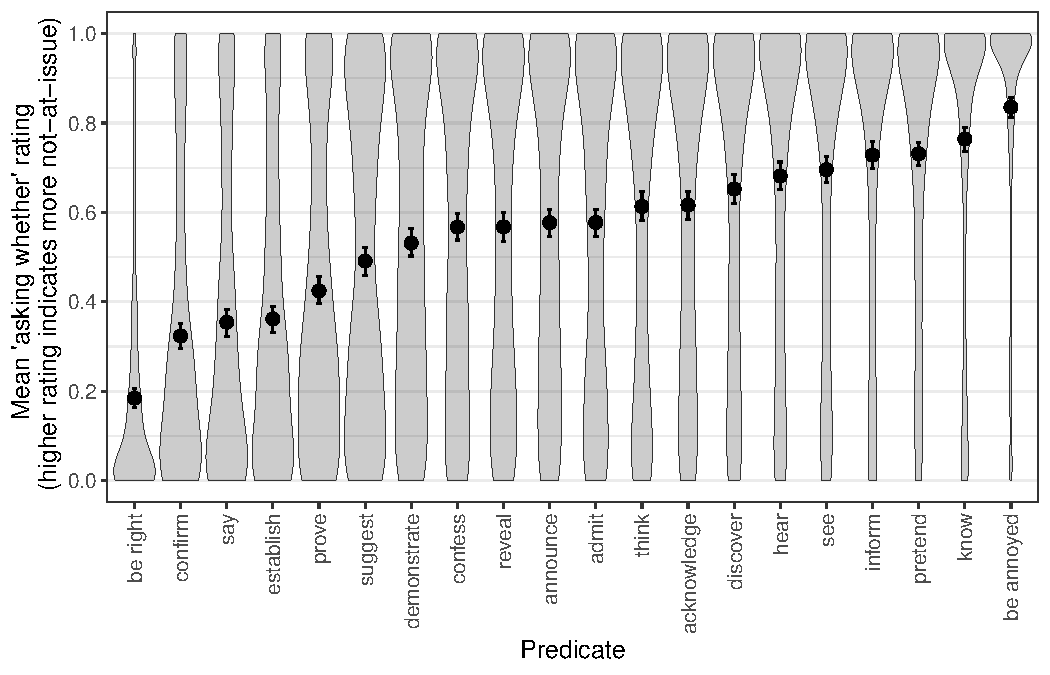
\includegraphics[width=0.7\textwidth]{../../results/main/degen-tonhauser-glossa/graphs/mean-asking-whether-ratings.pdf}

  \caption{Mean `asking whether' ratings for the contents of the clausal complements of 20 clause-embedding predicates, from \citealt{degen-tonhauser-glossa}.}
  \label{fig:dtglossa}
  \end{figure}

\section{Experiments 1-4 \label{sec:2_experiments}}

  To compare the results of at-issueness diagnostics, we conducted four experiments that each measured at-issueness with a different diagnostic, namely the QUD diagnostic (Exp.~1), the `asking whether' diagnostic (Exp.~2), the direct dissent diagnostic (Exp.~3) and the `yes, but' diagnostic (Exp.~4).\footnote{The experiments, data and R code for generating the figures and analyses of the experiments reported in this paper are available at INSERT URL TO ANONYMOUS GITHUB REPO BEFORE SUBMISSION. All experiments were conducted with approval from the ethics review committee of [university name redacted for review].} To be able to compare the results of the diagnostics, the same seven contents, shown in \ref{stims}, were investigated under the four diagnostics: the contents of sentence-medial and sentence-final NRRCs \ref{stims.a}-\ref{stims.b}, as well as the contents of the clausal complements of \emph{know, discover, confess, confirm} and \emph{be right} \ref{stims.c}-\ref{stims.g}. These seven contents were instantiated by the same items across the four experiments.

  \ex.\label{stims}
    \a.\label{stims.a} Content of sentence-medial NRRC \\
      \emph{Lucy, who broke the plate, apologised.} $\leadsto$ Lucy broke the plate
    \b.\label{stims.b} Content of sentence-final NRRC \\
    \emph{The police found Jack, who saw the murder.} $\leadsto$ Jack saw the murder
    \b.\label{stims.c} Content of the clausal complement of \emph{know} \\
    \emph{Ann knows that Raul cheated on his wife.} $\leadsto$ Raul cheated on his wife
    \b.\label{stims.d} Content of the clausal complement of \emph{discover} \\
    \emph{Mary discovered that Denny ate the last cupcake.} $\leadsto$ Denny ate the last cupcake
    \b.\label{stims.e} Content of the clausal complement of \emph{be right} \\
    \emph{Tom is right that Ann stole the money.} $\leadsto$ Ann stole the money
    \b.\label{stims.f} Content of the clausal complement of \emph{confirm} \\
    \emph{Harry confirmed that Greg bought a new car.} $\leadsto$ Greg bought a new car
    \b.\label{stims.g} Content of the clausal complement of \emph{confess}  \\
    \emph{Lucy confessed that Dustin lost his key.} $\leadsto$ Dustin lost his keys
    \z.
  \z.
  
These seven contents were chosen because prior literature observed differences in at-issueness between two or more of these contents using a particular diagnostic for at-issueness.  Specifically, as discussed in section \S1, \citealt{syrett_experimental_2015} observed differences between sentence-medial and -final NRRCs using a variant of the direct dissent diagnostic, \citealt{tonhauser_how_2018} observed differences between sentence-final NRRCs and the contents of the complements of \emph{know, discover} and \emph{confess} using the `asking whether' diagnostic, and \citealt{degen-tonhauser-glossa} observed differences between \emph{know, discover, confess, confirm} and \emph{be right}, also using the `asking whether' diagnostic. Thus, comparing these seven contents across the four diagnostics in Exps.~1-4 will allow us to assess whether the differences that emerge from one diagnostic also emerge from others. 

  In each experiment, participants read the stimuli and gave ratings corresponding to the diagnostics.

  \subsection{Methods}
    
  \subsubsection{Participants}

  For each of the four experiments, we recruited unique 80 participants on Prolific. These participants had registered on the platform as living in the USA and as having English as their primary language. They had at least 50 previous submissions and an approval rate of at least 97\%.  Table \ref{t:recruited} shows the age and gender distributions of the recruited participants.

  \begin{table}[h!]
  \centering
  \begin{tabular}{l | c | r r r }
              & recruited & ages (mean age) & f/m/nb/dnd \\ \hline
  Exp.~1 (QUD) & 80 & 18-81 (43.8) & 42/37/0/1  \\
  Exp.~2 (asking whether) & 80 & 20-74 (38.5)  & 48/30/1/1  \\
  Exp.~3 (direct dissent) & 80 & 18-77 (39.1) & 50/28/1/1  \\
  Exp.~4 (yes, but) &80 & 19-67 (38.0)  & 48/30/2/0 &  \\
  \hline
  \end{tabular}

  \caption{Information about the participants recruited in Exps.~1-4 (f = female, m = male, nb = nonbinary, dnd = did not disclose).}\label{t:recruited}
  \end{table}

  \subsubsection{Materials and procedure}
  
The four experiments measured the at-issueness of the seven contents in \ref{stims} with a different at-issueness diagnostic, namely the QUD diagnostic (Exp.~1), the `asking whether' diagnostic (Exp.~2), the direct dissent diagnostic (Exp.~3) and the `yes, but' diagnostic (Exp.~4). The examples in \ref{diag} illustrate how each diagnostic was implemented using the content of sentence-medial NRRCs (with the item `Lucy broke the plate'). In Exp.~1 (QUD diagnostic, \ref{diag.a}), participants read a dialogue between two named speakers, where the first utters an interrogative sentence (the presumed QUD) that is about the content to be diagnosed and the second responds with a declarative sentence that contributes the content to be diagnosed. In Exp.~2 (`asking whether' diagnostic, \ref{diag.b}), participants read an interrogative sentence uttered by a named speaker, where the interrogative sentence contributes the content to be diagnosed. In Exp.~3 (`direct dissent' diagnostic, \ref{diag.c}), participants read a dialogue between two named speakers, where the first utters a declarative sentence with the content to be diagnosed and the second directly dissents with the content to be diagnosed. Finally, in Exp.~4 (`yes, but' diagnostic, \ref{diag.d}), participants read a dialogue between two named speakers where the first utters a declarative sentence that contributes the content to be diagnosed and the second responds with one of two indirect dissent variants (\emph{yes, but..}, \emph{yes, and...}) or with a direct dissent.

\ex.\label{diag} Implementations of the diagnostics in Exps.~1-4
\a.\label{diag.a} Exp.~1 (QUD diagnostic)
\\ {\bf Nora:} \emph{What did Lucy break?}
\\ {\bf Leo:} \emph{Lucy, who broke the plate, apologized.}
\b.\label{diag.b} Exp.~2 (`asking whether' diagnostic )
\\ {\bf Nora:} \emph{Did Lucy, who broke the plate, apologize?}
\c.\label{diag.c} Exp.~3 (`direct dissent' diagnostic)
\\ {\bf Nora:} \emph{Lucy, who broke the plate, apologized.}
\\ {\bf Leo:} \emph{No, she didn't break the plate.}
\d.\label{diag.d} Exp.~4 (`yes, but' diagnostic)
\\ {\bf Nora:} \emph{Lucy, who broke the plate, apologized.}
\\ {\bf Nina:} \emph{Yes, but she didn't break the plate.}
\\ \hspace*{1cm} \emph{Yes, and she didn't break the plate.}
\\ \hspace*{1cm} \emph{No, she didn't break the plate.}

As shown in Fig.~\ref{fig:trials}, the response options in each of the four experiments differed depending on the diagnostic. In Exp.~1 (QUD diagnostic, panel (a)), participants were asked how well the response fits the question and they gave their response on a slider marked `totally doesn't fit' on one end (coded 0) and `totally fits' on the other end (coded as 1). In Exp.~2 (`asking whether' diagnostic, panel (b)), participants were asked whether the question is about the content to be diagnosed and they gave their response on a slider marked `no' on one end (coded as 1) and `yes' on the other (coded as 0). In Exp.~3 (direct dissent diagnostic, panel (c)), participants were asked how natural the direct dissent and participants gave their response on a slider marked `totally unnatural' (coded as 0) on one end and `totally natural' on the other (coded as 1). Finally, in Exp.~4 (`yes, but' diagnostic, panel (d)), participants were asked to choose the response that sounded best; the two indirect dissents were coded as 1 and the direct one as 0. Across the four experiments, the responses were coded as 0 or 1 in such a way that 0 meant that the content to be diagnosed was rated as at-issue and 1 meant that the content was rated as not-at-issue.


 \begin{figure}[h!]
  \centering
  % Top row
  \subfigure[Exp.~1: QUD diagnostic]{%
    \fbox{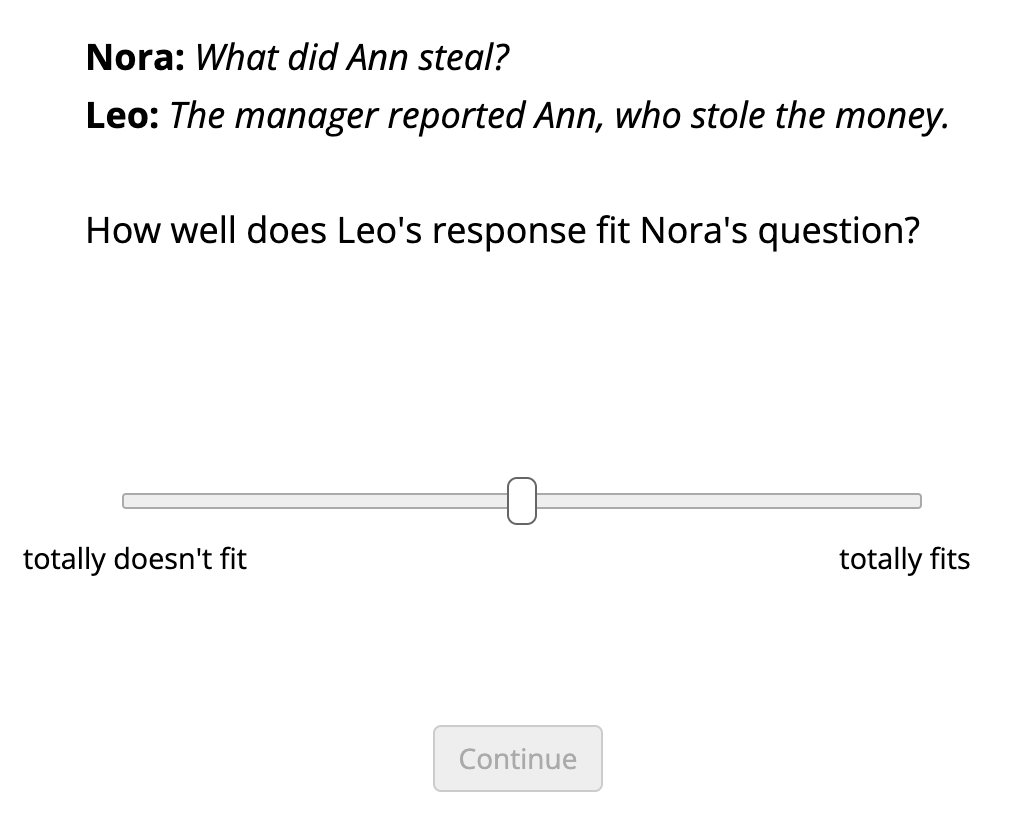
\includegraphics[width=0.47\textwidth]{figures/trialExp1}}%
    \label{fig:trialExp1}
  }
  \hfill
  \subfigure[Exp.~2: `asking whether' diagnostic]{%
    \fbox{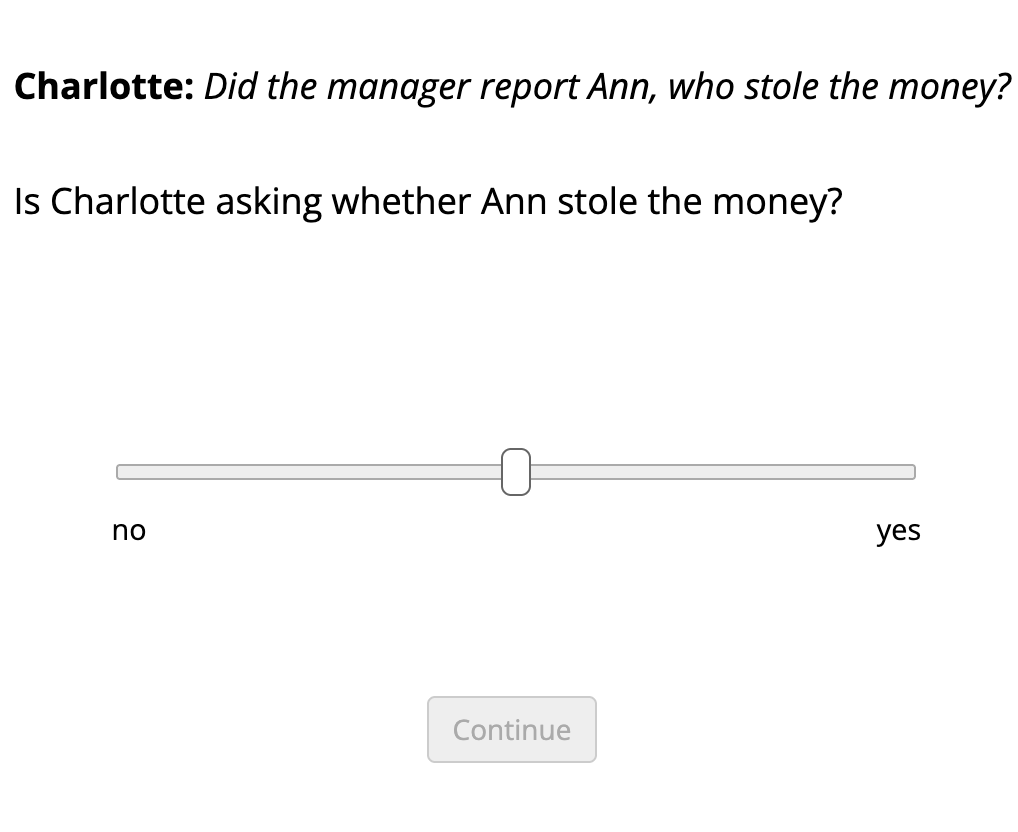
\includegraphics[width=0.47\textwidth]{figures/trialExp2}}%
    \label{fig:trialExp2}
  }

  \vspace{1em}

  % Bottom row
  \subfigure[Exp.~3: `direct dissent' diagnostic]{%
    \fbox{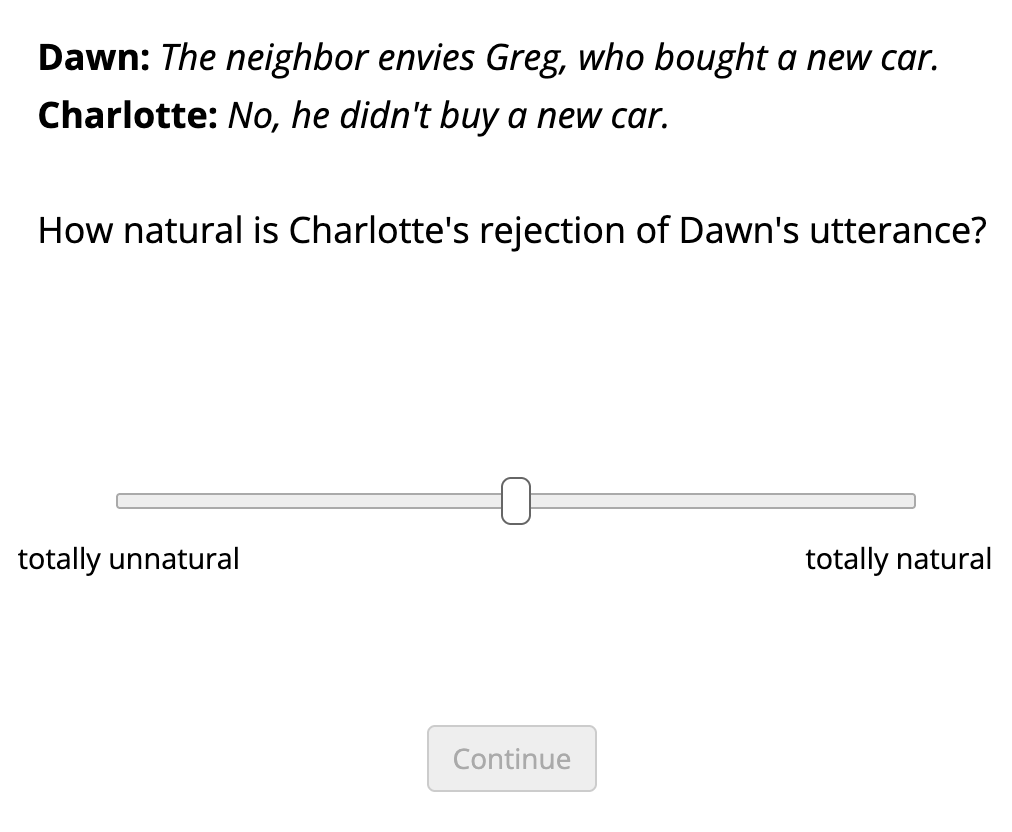
\includegraphics[width=0.47\textwidth]{figures/trialExp3}}%
    \label{fig:trialExp3}
  }
  \hfill
  \subfigure[Exp.~4: `yes, but' diagnostic]{%
    \fbox{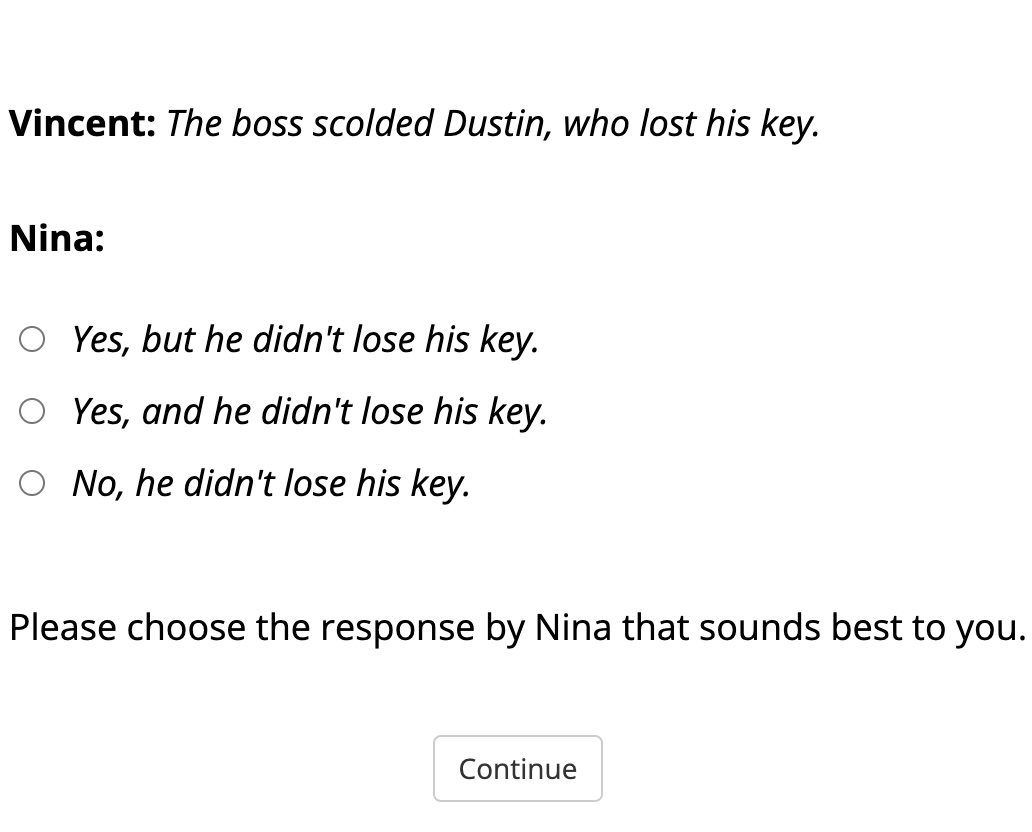
\includegraphics[width=0.47\textwidth]{figures/trialExp4}}%
    \label{fig:trialExp4}
  }

  \caption{Sample trials in (a) Exp.~1, (b) Exp.~2, (c) Exp.~3, and (d) Exp.~4.}
  \label{fig:trials}
  \end{figure}
  
  Each of the seven contents in \ref{stims} was instantiated by one of the seven items shown in \ref{items} in each of the four experiments.
 
 \ex.\label{items}
 \a. Jack saw the murder.
 \b. Raul cheated on his wife.
 \c. Ann stole the money.
 \d. Danny ate the last cupcake.
 \b. Lucy broke the plate.
 \b. Dustin lost his key.
 \b. Greg bought a new car.
 \z.
 
 Each experiment also included two control stimuli, which functioned as attention checks: one stimulus was expected to receive a response at one end of the slider (Exps.~1-3) or a `no' response (Exp.~4); the other control stimulus was expected tor receive a response at the other end of the slider (Exps.~1-3) or a `yes' response (Exp.~4). See Supplement \ref{supp:stims} for the control stimuli used in Exps.~1-4.
 
 In each of the four experiments, each participant's set of items was generated by randomly combining each of the seven contents in \ref{stims} with a unique content in \ref{items}. Participants completed a total of 9 trials, namely 7 target trials and the same 2 control trials. Trial order was randomized.
 
After completing the experiment, participants filled out a short optional demographic survey. To encourage truthful responses, participants were told that they would be paid no matter what answers they gave in the survey. 

  \subsubsection{Data exclusion}
    
  We excluded the data of participants who did not self-identify as native speakers of
  American English and of participants whose responses to either one of the two control trials was more than 2 sd away from the group mean (Exps.~1-3) or whose responses to either one of the two control trials was wrong (Exp.~4).   Table \ref{t:excluded} shows how many participants were excluded in each experiment, the properties of the remaining participants, and the number of data points that entered into the analyses.

  \begin{table}[h!]
  \centering
  \begin{tabular}{l | r r | r r  | r }
               & \multicolumn{2}{c|}{\bf exclusion criterion} & \multicolumn{2}{c|}{\bf remaining participants} & data \\ 
              & language & fillers & ages (mean age) & f/m/nb/dnd &  points \\ \hline
  Exp.~1 (QUD   & 1 &  10 &  18-81 (41.1) & 36/32/0/1 & 621 \\ 
  Exp.~2 (asking whether) &  2 &  4 & 22-74 (38.7) & 45/27/1/1 & 666 \\ 
  Exp.~3  (direct dissent) &  2 &  7 & 18-77 (39.5) & 44/25/1/1  & 639 \\ 
  Exp.~4  (yes, but) & 4 & 4 & 19-67 (38.5)  & 43/27/2/0 & 648 \\ 
  \hline
  \end{tabular}
  \caption{Information from Exps.~1-4 about the number of participants whose data was excluded based on their self-declared language (variety) and the fillers, about the remaining participants, and about the number of data points that entered into the analysis.}\label{t:excluded}
  \end{table}

  \subsection{Results}
  
  Fig.~\ref{fig:results} plots the results of the four experiments by the expression that is associated with the seven target contents {\bf and the two controls}\footnote{given that the controls do not all tell us something useful about at-issueness, I suggest we remove them from the plots; we also don't need them to discuss the results; need to make the expressions identical across the four panels}: panel (a) shows the mean naturalness ratings in Exp.~1 (QUD diagnostic), panel (b) the mean `asking whether' ratings in Exp.~2 (`asking whether' diagnostic), panel (c) the mean naturalness ratings in Exp.~3 (`direct dissent' diagnostic) and panel (d) the proportion of `no' choices in Exp.~4 (`yes, but' diagnostic). Two differences between the results of the four experiments concern the relative rankings between the seven contents in each experiment and the extent to which the experiments differentiate between the seven contents. 
  
  Regarding the first difference, we observe that the relative ranking of the seven contents differs between the four experiments. The only pair of contents that are ranked the same way across all four experiments are the content of the complement of \emph{discover}, which received higher ratings (at least numerically) across all four experiments than that of \emph{confess}. There is no other pair of expressions for which that is the case. For instance, whereas the content of the complement of \emph{confirm} received (numerically) higher ratings than that of \emph{know} in Exps.~1 and 2, the opposite pattern is observed in Exps.~3 and 4. This difference between the experiments is quantified in the Spearman rank correlations in Table \ref{t:spearman},\footnote{The Spearman rank correlation coefficient, a value between -1 and 1, is a nonparametric measure of rank correlation: the higher the coefficient, the more the relation between the the two variables can be described using a monotonic function. If the coefficient is positive, the value of one variable tends to increase with an increase in the other. In the case of our experiments, a coefficient of 1 for two experiments would mean that there is a perfectly monotone increasing relation between the mean ratings of the seven contents in the two experiments: for any two contents c1 and c2, if c1 ranks below c2 in one experiment (that is, the mean rating of c1 is lower than that of c2), then that ranking is preserved in the other experiment.} which are particularly low for Exp.~1 compared to the other three experiments. This is due, to some extent, to the content of the complement of \emph{be right} being ranked the lowest in Exp.~1 but among the highest in Exps.~2-4.\footnote{When \emph{be right} is excluded, the Spearman rank correlations are:
  
 \begin{tabular}{l | c c c c}
 & Exp.~1 & Exp.~2 & Exp.~3 & Exp.~4 \\ \hline
 Exp.~1 (QUD diagnostic) & \cellcolor{lightgray} & .77 & .09 & .31 \\
 Exp.~2 (`asking whether' diagnostic) & \cellcolor{lightgray} & \cellcolor{lightgray} & .66 & .66 \\
 Exp.~3 (`direct dissent' diagnostic) & \cellcolor{lightgray}& \cellcolor{lightgray} & \cellcolor{lightgray} & .77  \\
 \hline
% Exp.~4 (`yes, but' diagnostic) & & & & \cellcolor{lightgray} \\ \hline
 \end{tabular}} {\bf discuss be right here!} This result suggests that the four diagnostics as implemented in Exps.~1-4 interact differently with the seven contents investigated.
 
 \begin{table}[ht!]
 \centering
 \begin{tabular}{l | c c c c}
 & Exp.~1 & Exp.~2 & Exp.~3 & Exp.~4 \\ \hline
 Exp.~1 (QUD diagnostic) & \cellcolor{lightgray} & .11 & -.29 & -.18 \\
 Exp.~2 (`asking whether' diagnostic) & \cellcolor{lightgray} & \cellcolor{lightgray} & .64 &.79 \\
 Exp.~3 (`direct dissent' diagnostic) & \cellcolor{lightgray}& \cellcolor{lightgray} & \cellcolor{lightgray} & .79  \\
 \hline
% Exp.~4 (`yes, but' diagnostic) & & & & \cellcolor{lightgray} \\ \hline
 \end{tabular}
 \caption{Spearman rank correlations between the results of Exps.~1-4.}\label{t:spearman}
 \end{table}
  
 
  \begin{figure}[h!]
    \centering

    % Top row
    \subfigure[Exp.~1 (QUD diagnostic)]{%
      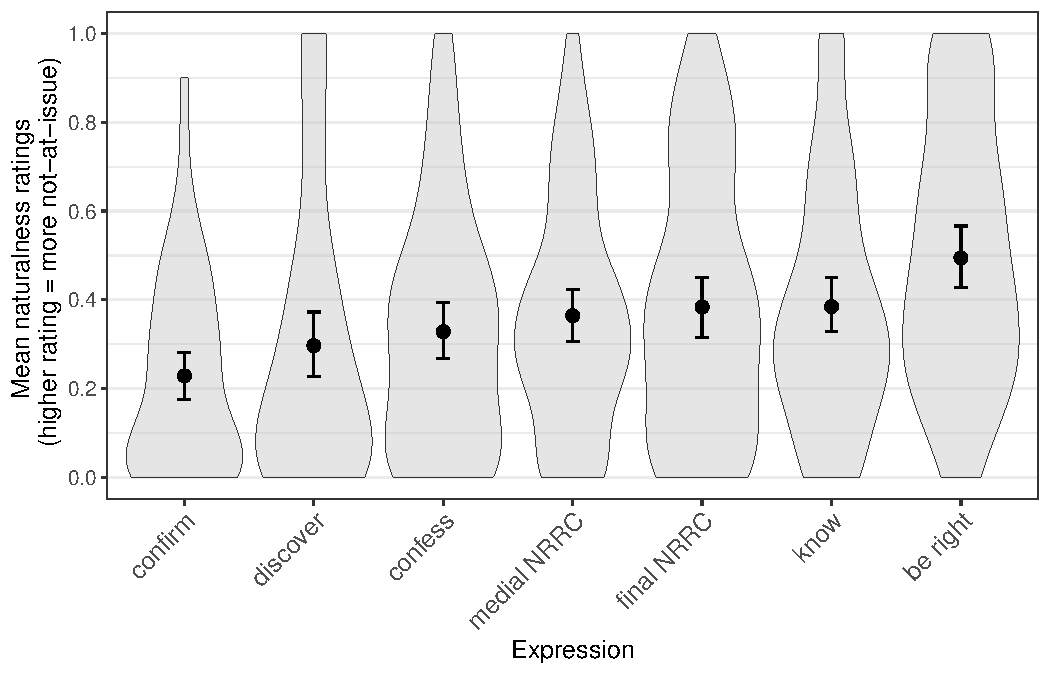
\includegraphics[width=0.48\linewidth]{../../results/main/exp1/graphs/mean-ratings.pdf}%
      \label{fig:qud}
    }
    \hfill
    \subfigure[Exp.~2 (`asking whether' diagnostic)]{%
      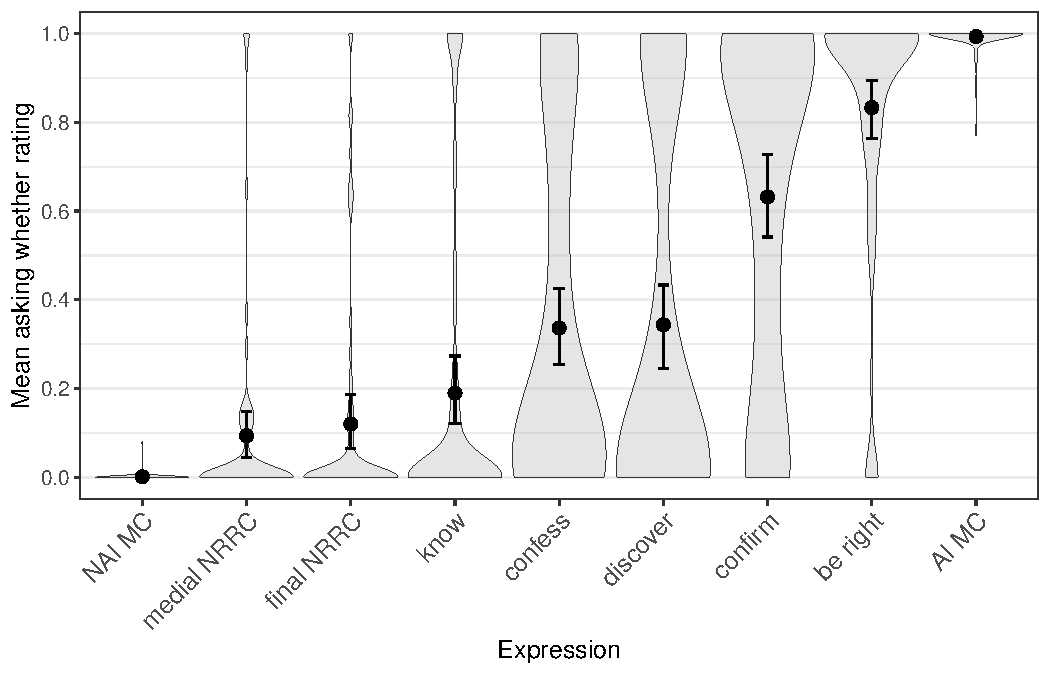
\includegraphics[width=0.48\linewidth]{../../results/main/exp2/graphs/mean-ratings.pdf}%
      \label{fig:AK}
    }

%    \vspace{1em}

    % Bottom row
    \subfigure[Exp.~3 (`direct dissent' diagnostic)]{%
      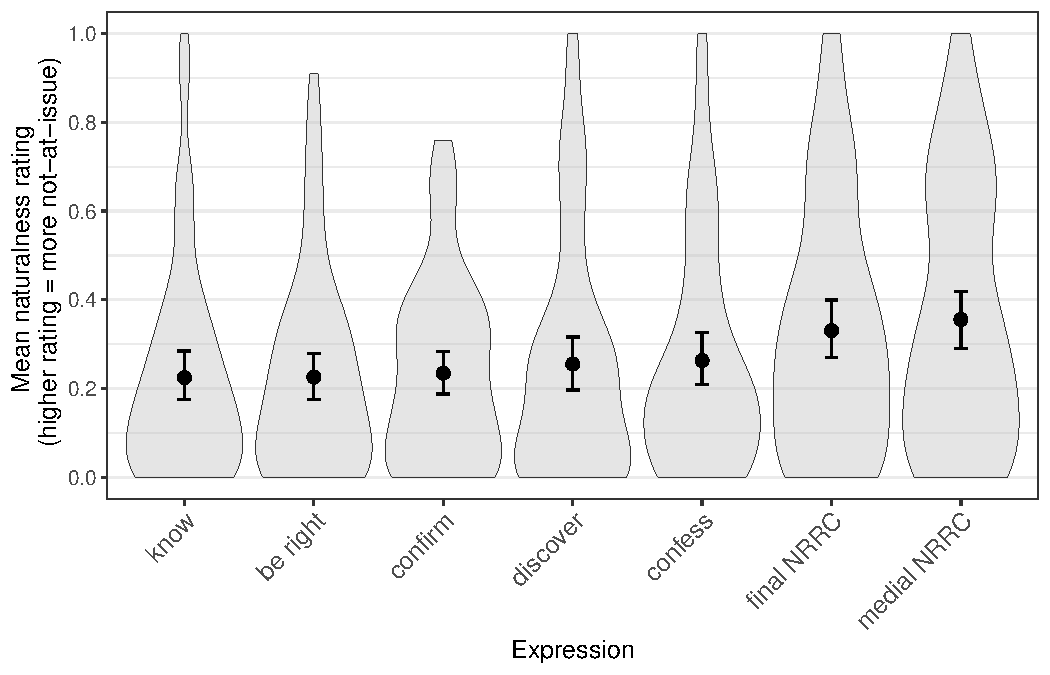
\includegraphics[width=0.48\textwidth]{../../results/main/exp3/graphs/mean-ratings.pdf}%
      \label{fig:dd}
    }
    \hfill
    \subfigure[Exp.~4 (`yes, but' diagnostic)]{%
      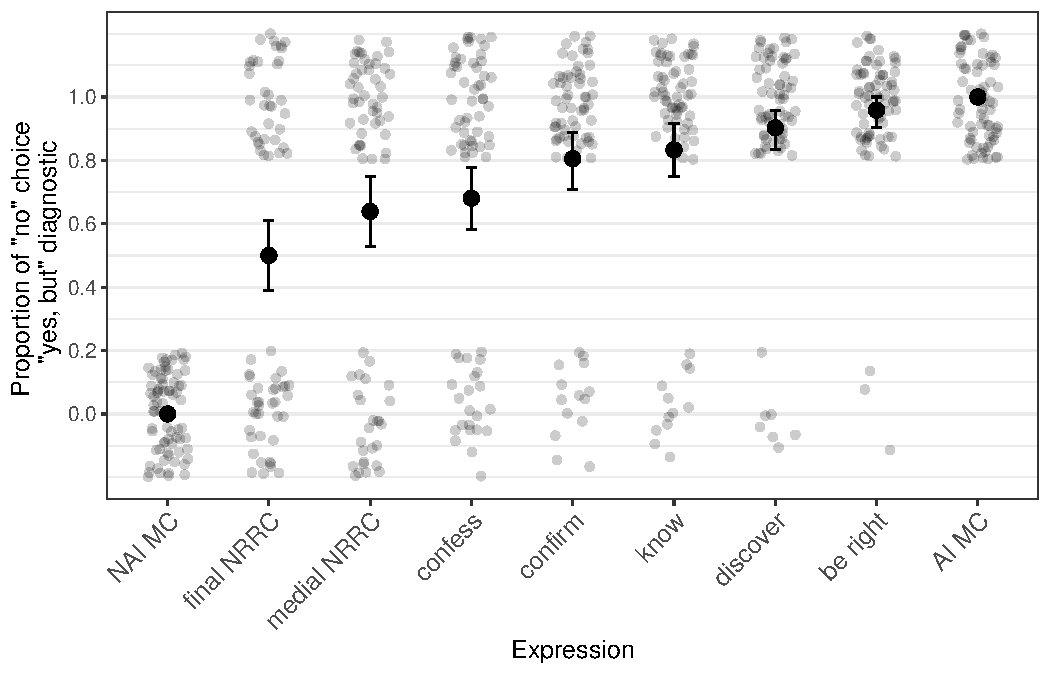
\includegraphics[width=0.48\textwidth]{../../results/main/exp4/graphs/mean-ratings.pdf}%
      \label{fig:yb}
    }

    \caption{Results of Exps.~1--4. Panels (a)--(c) show the mean responses by expression for (a) Exp.~1 (QUD diagnostic),  (b) Exp.~2 (`asking whether' diagnostic), and (c) Exp.~3 (`direct dissent' diagnostic); panel (d) shows the proportion of `no' choices by expression in Exp.~4 (`yes, but' diagnostic). Error bars indicate 95\% bootstrapped confidence intervals. Violin plots in panels (a)-(c) show the kernel probability density of individual participants' ratings. Gray dots in panel (d) represent individual participant responses (`no' vs.\ `yes', jittered vertically and horizontally for legibility).}
    \label{fig:results}
  \end{figure}
  
Regarding the second difference, we consider the range of (mean or proportion of) ratings, that is, the difference between the largest and smallest ratings. The range is largest in Exp.~2 (`asking whether' diagnostic), at .74 (.01 to .83) and smallest in Exp.~3 (`direct dissent' diagnostic), at .13 (.64 to .78). The results of Exp.~1 (QUD diagnostic, with a range of .27 (.51 to .77) and Exp.~4 (`yes, but' diagnostic), with a range of .46 (.5 to .96), fall in-between. This result suggests that the four diagnostics as implemented in Exps.~1-4 differ in how much they differentiate between the seven contents investigated, with the `asking whether' diagnostic showing the most differentiation and the `direct dissent' and the QUD diagnostic showing the least differentiation.
  
 %Exp 1
 %min: 0.5055072
 %max: 0.7713043
 %range: 0.2657971
 
 %Exp 2
 %min: 0.09364865
 %max: 0.8332432
 %range: 0.7395946
 
 %Exp 3
 %min: 0.6443662
 %max: 0.7752113
 %range: 0.1308451
  
 %Exp 4
 %min: .5
 %max: 0.958
 %range: 0.458
 
This observation is supported by the results of post hoc pairwise comparisons using Tukey's method (allowing for by-participant variability), using the `lsmeans' package (\citealt{tukey}) in R.

{\bf NEED Different colors because directions of differences vary!}

\addtolength{\tabcolsep}{-.19em}

\begin{figure}[!h]
\centering

\subfigure[Exp.~1 (QUD diagnostic)]{%
\begin{tabular}{r | ccccccc}
& \rots{be right} & \rots{confess} & \rots{confirm} & \rots{discover} & \rots{final NRRC} & \rots{know} & \rots{medial NRRC} \\
\hline
 be.right & \cellcolor{black} & \cellcolor{gray} & \cellcolor{gray} & \cellcolor{gray} & \cellcolor{gray} & \cellcolor{gray} & \cellcolor{gray} \\ 
  confess & \cellcolor{gray} & \cellcolor{black} & \cellcolor{gray} & \cellcolor{white} & \cellcolor{white} & \cellcolor{white} & \cellcolor{white} \\ 
  confirm & \cellcolor{gray} & \cellcolor{gray} & \cellcolor{black} & \cellcolor{gray} & \cellcolor{gray} & \cellcolor{gray} & \cellcolor{gray} \\ 
  discover & \cellcolor{gray} & \cellcolor{white} & \cellcolor{gray} & \cellcolor{black} & \cellcolor{gray} & \cellcolor{white} & \cellcolor{white} \\ 
  final NRRC & \cellcolor{gray} & \cellcolor{white} & \cellcolor{gray} & \cellcolor{gray} & \cellcolor{black} & \cellcolor{white} & \cellcolor{white} \\ 
  know & \cellcolor{gray} & \cellcolor{white} & \cellcolor{gray} & \cellcolor{white} & \cellcolor{white} & \cellcolor{black} & \cellcolor{white} \\ 
  medial NRRC & \cellcolor{gray} & \cellcolor{white} & \cellcolor{gray} & \cellcolor{white} & \cellcolor{white} & \cellcolor{white} & \cellcolor{black} \\ 
  

\hline
\end{tabular}}
\hfill
\subfigure[Exp.~2 (`asking whether' diagnostic)]{%
\begin{tabular}{r | ccccccc}
& \rots{be right} & \rots{confess} & \rots{confirm} & \rots{discover} & \rots{final NRRC} & \rots{know} & \rots{medial NRRC} \\
\hline
 be right & \cellcolor{black} & \cellcolor{blue} & \cellcolor{blue} & \cellcolor{blue} & \cellcolor{blue} & \cellcolor{blue} & \cellcolor{blue} \\ 
  confirm & \cellcolor{black} & \cellcolor{black} & \cellcolor{blue} & \cellcolor{blue} & \cellcolor{blue} & \cellcolor{blue} & \cellcolor{blue} \\ 
  discover & \cellcolor{black} & \cellcolor{black} & \cellcolor{black} & \cellcolor{white} & \cellcolor{blue} & \cellcolor{blue} & \cellcolor{blue} \\ 
  confess & \cellcolor{black} & \cellcolor{black} & \cellcolor{black} & \cellcolor{black} & \cellcolor{blue} & \cellcolor{blue} & \cellcolor{blue} \\ 
  know & \cellcolor{black} & \cellcolor{black} & \cellcolor{black} & \cellcolor{black} & \cellcolor{black} & \cellcolor{blue} & \cellcolor{blue} \\ 
  final NRRC & \cellcolor{black} & \cellcolor{black} & \cellcolor{black} & \cellcolor{black} & \cellcolor{black} & \cellcolor{black} & \cellcolor{white} \\ 
  medial NRRC & \cellcolor{black} & \cellcolor{black} & \cellcolor{black} & \cellcolor{black} & \cellcolor{black} & \cellcolor{black} & \cellcolor{black} \\ 
  

\hline
\end{tabular}}

\subfigure[Exp.~3 (`direct dissent' diagnostic)]{%
\begin{tabular}{r | ccccccc}
& \rots{be right} & \rots{confess} & \rots{confirm} & \rots{discover} & \rots{final NRRC} & \rots{know} & \rots{medial NRRC} \\
\hline
 be.right & \cellcolor{black} & \cellcolor{gray} & \cellcolor{gray} & \cellcolor{gray} & \cellcolor{gray} & \cellcolor{gray} & \cellcolor{gray} \\ 
  confess & \cellcolor{gray} & \cellcolor{black} & \cellcolor{gray} & \cellcolor{white} & \cellcolor{white} & \cellcolor{white} & \cellcolor{white} \\ 
  confirm & \cellcolor{gray} & \cellcolor{gray} & \cellcolor{black} & \cellcolor{gray} & \cellcolor{gray} & \cellcolor{gray} & \cellcolor{gray} \\ 
  discover & \cellcolor{gray} & \cellcolor{white} & \cellcolor{gray} & \cellcolor{black} & \cellcolor{gray} & \cellcolor{white} & \cellcolor{white} \\ 
  final NRRC & \cellcolor{gray} & \cellcolor{white} & \cellcolor{gray} & \cellcolor{gray} & \cellcolor{black} & \cellcolor{white} & \cellcolor{white} \\ 
  know & \cellcolor{gray} & \cellcolor{white} & \cellcolor{gray} & \cellcolor{white} & \cellcolor{white} & \cellcolor{black} & \cellcolor{white} \\ 
  medial NRRC & \cellcolor{gray} & \cellcolor{white} & \cellcolor{gray} & \cellcolor{white} & \cellcolor{white} & \cellcolor{white} & \cellcolor{black} \\ 
  

\hline
\end{tabular}}
\hfill
\subfigure[Exp.~4 (`yes, but' diagnostic)]{%
\begin{tabular}{r | ccccccc}
& \rots{be right} & \rots{confess} & \rots{confirm} & \rots{discover} & \rots{final NRRC} & \rots{know} & \rots{medial NRRC} \\
\hline
 be right & \cellcolor{black} & \cellcolor{blue} & \cellcolor{blue} & \cellcolor{blue} & \cellcolor{blue} & \cellcolor{blue} & \cellcolor{blue} \\ 
  confirm & \cellcolor{black} & \cellcolor{black} & \cellcolor{blue} & \cellcolor{blue} & \cellcolor{blue} & \cellcolor{blue} & \cellcolor{blue} \\ 
  discover & \cellcolor{black} & \cellcolor{black} & \cellcolor{black} & \cellcolor{white} & \cellcolor{blue} & \cellcolor{blue} & \cellcolor{blue} \\ 
  confess & \cellcolor{black} & \cellcolor{black} & \cellcolor{black} & \cellcolor{black} & \cellcolor{blue} & \cellcolor{blue} & \cellcolor{blue} \\ 
  know & \cellcolor{black} & \cellcolor{black} & \cellcolor{black} & \cellcolor{black} & \cellcolor{black} & \cellcolor{blue} & \cellcolor{blue} \\ 
  final NRRC & \cellcolor{black} & \cellcolor{black} & \cellcolor{black} & \cellcolor{black} & \cellcolor{black} & \cellcolor{black} & \cellcolor{white} \\ 
  medial NRRC & \cellcolor{black} & \cellcolor{black} & \cellcolor{black} & \cellcolor{black} & \cellcolor{black} & \cellcolor{black} & \cellcolor{black} \\ 
  

\hline
\end{tabular}}

\caption{Pairwise differences between expressions (ordered from top to bottom and left to right by increasing mean in Exp.~2 (`asking whether' diagnostic). A gray cell for a pair means that the 95\% HDI did not include 0; a white cell means that the 95\% HDI included 0.}\label{fig:pairwise}
\end{figure}


\subsection{Discussion}

Confound wrt be right should be discussed here

    The differening results between diagnostics suggest that they are not interchangeable.

    \subsubsection{Sensitivity}

      \begin{itemize}
        \item Further, while the `asking whether' diagnostic, for contents embedded in questions, is sensitive enough to detect fine-grained differences between contents, the smaller range of response means for the other diagnostics could suggest the need for a more sensitive diagnostic for contents embedded in declarative assertions.

        \item We did not replicate the effect reported in \citealt{syrett_experimental_2015}, that sentence-final NRRCs receive higher at-issueness ratings than sentence-medial ones.

        \item  Additional comparison to \citealt{syrett_experimental_2015} (details omitted in the abstract) points to potential effects of the response task and the speech act of the utterance embedding the tested content.

      \end{itemize}

    \subsubsection{Order}

      \begin{itemize}
        \item In particular, the varying relative order of by-content means across diagnostics provide an initial argument that they target distinct properties of the content.
      \end{itemize}
      
      
\section{Experiments 5-6}

\subsection{Methods}

\subsection{Results}

\subsection{Discussion}

\section{General discussion}



\section{Conclusion}

The conclusion is the last numbered section, and any ensuing sections are unnumbered.

\pagebreak
\section*{Abbreviations (if applicable)}\label{abbrev}

\textsc{acc} = accusative, \textsc{dat} = dative, \textsc{dem} = demonstrative, \textsc{nom} = nominative, \textsc{pl} = plural, \textsc{sg} = singular

For the standard abbreviations to be used here, refer to the \href{https://www.eva.mpg.de/lingua/resources/glossing-rules.php}{Leipzig glossing rules}.

\section*{Data availability/Supplementary files (if applicable)}

The journal encourages authors to make all data associated with their submission openly available, according to the FAIR principles (Findable, Accessible, Interoperable, Reusable). More information can be found \href{https://www.glossa-journal.org/site/editorial-policies/#data-policy}{here}.

If data/supplementary files are to be associated with the accepted paper, one of the options below should be followed:
\begin{enumerate}
\item upload the files to your chosen open repository and make note of the DOI that they will provide (most suitable for datasets or information that act as foundations to the research being published. This option makes the files more findable and more citable). We recommend an open repository such as osf.io, which allows you to create a "project" under which you can upload relevant files (datasets, analysis scripts, experimental materials, etc.). The project will be associated with a unique DOI. You can then include in your manuscript a citation of the OSF entry and/or a link to the project page on OSF, to direct interested readers to the supplementary materials. During review, please be sure that the link to the repository is anonymized to maintain a fully double masked review process. Instructions for doing this on the OSF may be found \href{https://help.osf.io/hc/en-us/articles/360019930333-Create-a-View-only-Link-for-a-Project}{here}. If you'd like to learn more about best practices for ensuring reproducibility, see \href{https://psyarxiv.com/hf297/}{Laurinavichyute and Vasishth (2021)}. Please contact us if you would like more information or advice about hosting your data on an open repository.
\item upload the files to the journal system during the submission process, as `data files'. The journal will then host them as part of the publication and provide them with a DOI (most suitable for non-data files or very short pieces of information, although option 1 is also suitable for these if the author prefers).
\end{enumerate}

\noindent In both cases, a `Data availability' or `Supplementary files' section must be added prior to the reference list that provides a title and very short summary of the files for each file. If option 1 was selected, you should also provide the DOI in this section. For example:

\noindent Supplementary file 1: Appendix. Scientific data related to the experiments. DOI: \doi{10.5334/gjgl.310.s1}

Ideally, supplementary files are also cited in the main text.

Please note that neither of the above two options will result in the files being typeset, so please ensure that they are in publishable format when you upload the accepted paper.


\section*{Ethics and consent (if applicable)}

Research involving human subjects, human material, or human data, must have been performed in accordance with the Declaration of Helsinki. Studies must have been approved by an appropriate ethics committee and the authors should include a statement in the article text detailing this approval, including the name of the ethics committee and reference number of the approval, or mention any exemptions to ethical approval that apply to their research. The identity of research subjects should be anonymised whenever possible. For research involving human subjects, informed consent to participate in the study must be obtained from participants (or their legal guardian).


\section*{Funding information (if applicable)}

Should the research have received a funding grant then the grant provider and grant number should be detailed.

\section*{Acknowledgements (optional)}

The authors wish to thank Martin Haspelmath for providing the generic style sheet for linguistics, and Kai von Fintel for giving permission to use and modify the \textit{Semantics \& Pragmatics} Latex template, bibliography style, and document class.

\section*{Competing interests (required)}

If any of the authors have any competing interests then these must be declared. Guidelines for competing interests can be found \href{https://www.glossa-journal.org/site/competing-interests/}{here}. If there are no competing interests to declare then the following statement should be present: `The author(s) has/have no competing interests to declare'.

\section*{Authors' contributions (optional)}\label{contrib}

A sentence or a short paragraph detailing the roles that each author held to contribute to the authorship of the submission.  Individuals listed must fit within the definition of an author, as per our \href{https://www.glossa-journal.org/site/author-guidelines/}{Author Guidelines}.

\nocite{*} %this is to get all the entries of the sample bibliography; delete this line for an actual Glossa submission

%\printbibliography %for use with biblatex; comment out if you use natbib
\bibliography{../at-issueness} %for use with natbib; comment out if you use biblatex, and change 'sample' by the name of your bib-file


\appendix

\setcounter{table}{0}
\renewcommand{\thetable}{A\arabic{table}}

\setcounter{figure}{0}
\renewcommand{\thefigure}{A\arabic{figure}}

\setcounter{ExNo}{0}


\section*{Supplements}

\section{Control stimuli in Exps.~1-4}\label{supp:stims}

The examples in \ref{control1}-\ref{control4} provide the two control stimuli used in each of Exps.~1-4. For the a.-examples, participants were expected to give a `totally fits' response (Exp.~1), a `yes' response (Exp.~2), a `totally natural' response (Exp.~3), and a `no' response (Exp.~4); for the b.-examples, the opposite response was expected. The numbers  after each example identify the mean ratings (Exps.~1-3) or the proportion of `no' responses (Exp.~4) after excluding participants who did not self-identify as native speakers of American English (but before excluding participants on the basis of these controls), showing that the control stimuli worked as intended.

\ex.\label{control1} Control stimuli in Exp.~1 (QUD diagnostic)
\a. Mary: Which course did Ava take?
\\ John: She took the French course. (.97)
\b. Jennifer: What does Betsy have?
\\ Robert: She loves dancing salsa. (.07)

\ex.\label{control2} Control stimuli in Exp.~2 (`asking whether' diagnostic)
\a. Mary: Did Arthur take a French course?
\\ Question to participants: Is Mary asking whether Arthur took a French course? (.96)
\b. Robert: Does Betsy have a cat?
\\ Question to participants: Is Robert asking whether Betsy loves apples? (.02)

\ex.\label{control3} Control stimuli in Exp.~3 (`direct dissent' diagnostic)
\a. Mary: Arthur took a French course.
\\ Lily: No, he took a Spanish course. (.87)
\b. Robert: Betsy has a cat.
\\ Maximilian: No, she doesn't like apples. (.05)

\ex.\label{control4} Control stimuli in Exp.~4 (`yes, but' diagnostic)
\a. Mary: Arthur took a French course.
\\ Lily: Yes, but Lisa loves cats. / Yes, and he didn't take a French course. / No, he didn't take a French course. (.95)
\b. Robert: Betsy has a cat.
\\ Maximilian: Yes, but she is good at math. / Yes, and she loves it so much. / No, she doesn't like apples. (0)

\end{document}
%%% Local Variables:
%%% mode: latex
%%% TeX-master: t
%%% TeX-engine: luatex
%%% End:
